\section{Introduction}

A desired capability of intelligent embodied agents is to rapidly adapt to new scenarios through experience.
An essential requirement for this capability is integrating a long history of experience into decision-making to enable an agent to accumulate knowledge about the new scenario that it is encountering.
For example, a robot placed in an unseen house initially has no knowledge of the home layout and where to find objects.
The robot should leverage its history of experiences of completing tasks in this new home to learn the home layout details, where to find objects, and how to act to complete tasks successfully.

To achieve adaptation of decision-making to new tasks, prior work has leveraged a technique called in-context reinforcement learning (RL) where an agent is trained with RL to utilize past experience in an environment~\citep{wang2016learning,team2023human,duan2016rl,grigsby2023amago,melo2022transformers}. 
By using sequence models over a history of interactions in an environment, these methods adapt to new scenarios by conditioning policy actions on this context of interaction history without updating the policy parameters.
While in-context RL has demonstrated the ability to scale to a context length of a few thousand 
agent steps~\citep{team2023human,grigsby2023amago}, this falls short of the needs of embodied AI where single tasks by themselves can span thousands of steps~\citep{szot2021habitat}. 
As a result, the agent cannot learn from multiple task examples because the context required for multiple tasks cannot be accommodated within the policy context.
Furthermore, prior work typically focuses on non-visual tasks~\citep{grigsby2023amago,melo2022transformers,ni2023transformers}, where larger histories are easier to incorporate due to the compact state representation.

In this work, we propose a new algorithm for in-context RL, which enables effectively utilizing and scaling to 64,000 steps of in-context experience in partially observable, visual navigation tasks. 
Our proposed method called \Method (\method), achieves this by leveraging a novel update and data collection technique for training with long training contexts in on-policy RL.
Using a long context for existing RL algorithms is prohibitively sample inefficient, as the agent must collect an entire long context of experience before updating the policy.
In addition, the agent struggles to utilize the experience from long context windows due to the challenge of learning long-horizon credit assignment and high-dimensional visual observations.
To address this problem, we introduce ``partial updates" where the policy is updated multiple times within a long context rollout over increasing context window lengths. 
We also introduce \sinkv to further increase context utilization by enabling more flexible attention over long sequences by adding learnable \textit{sink key and value} vectors to each attention layer.
These learned vectors are prepended to the input's keys and values in the attention operation. 
\sinkv stabilizes training by enabling the agent to not attend to low information observation sequences. 

\begin{figure*}[!t]
    \centering
    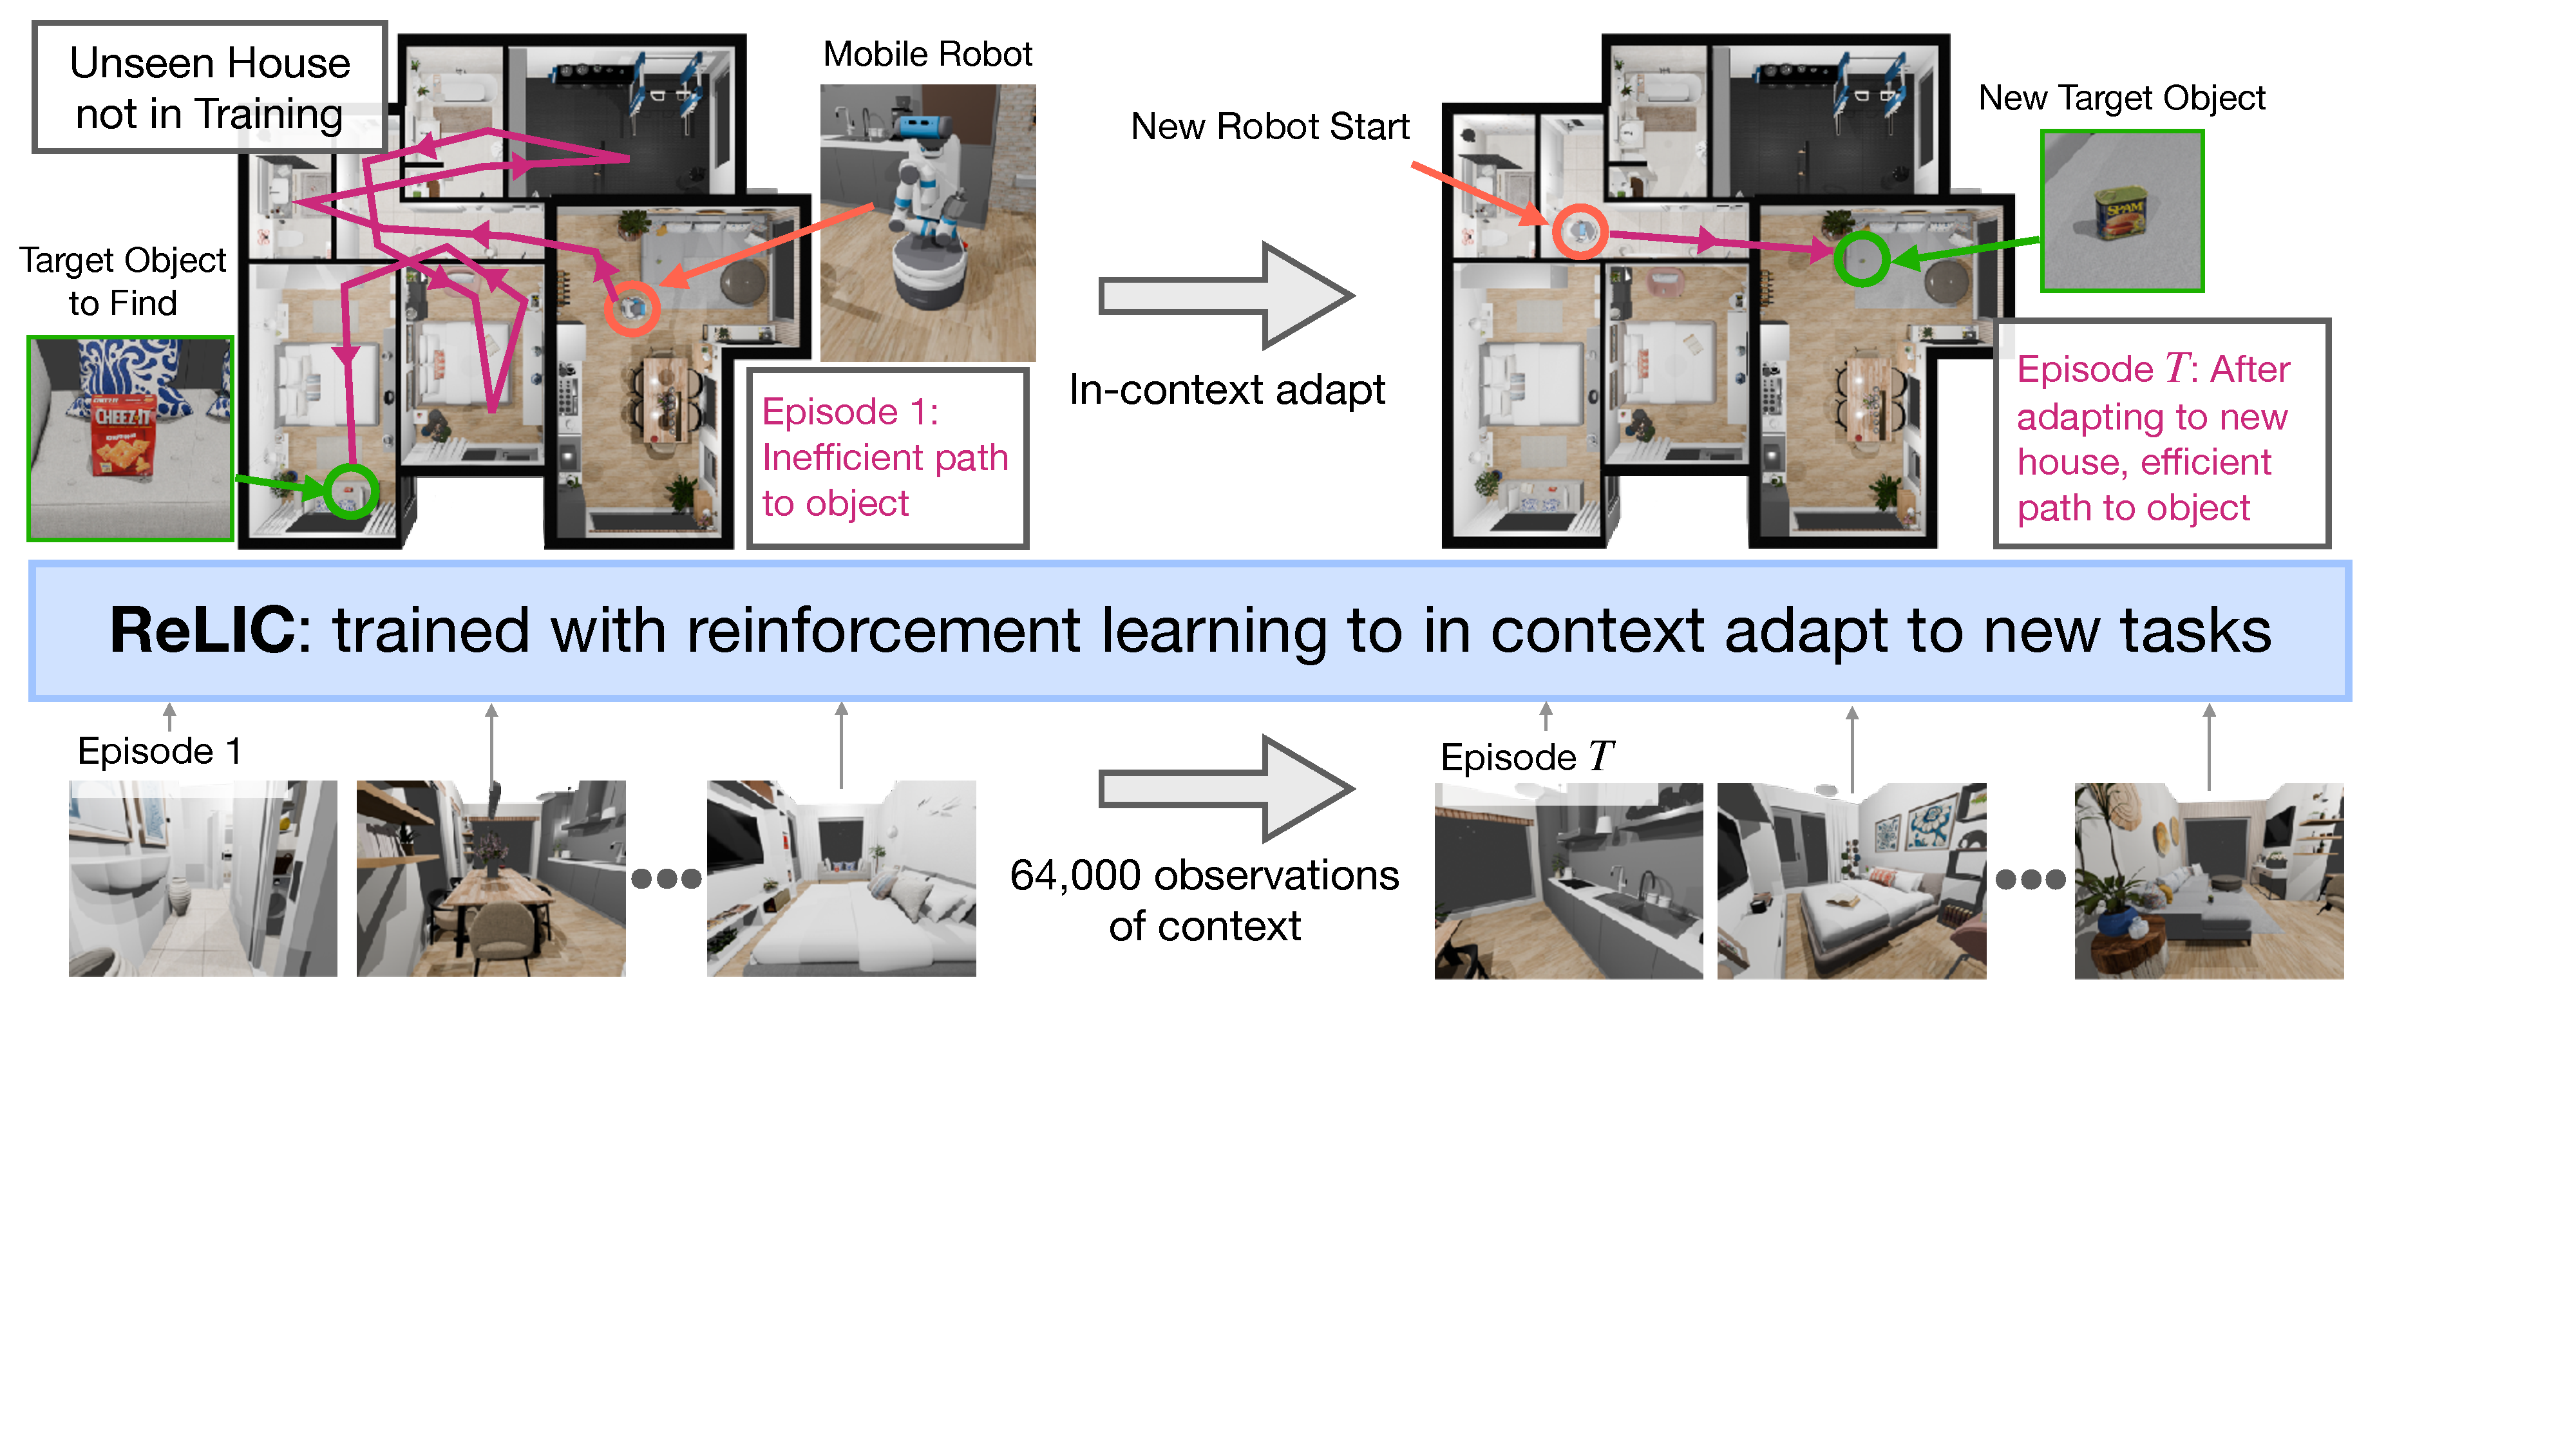
\includegraphics[width=\textwidth]{figures/diagrams/teaser.pdf}
    \caption{
        Overview of the \method approach and problem setup. \method learns a ``pixels-to-actions" policy from reward alone via reinforcement learning capable of in-context adapting to new tasks at test time. The figure shows the trained \method policy finding objects in an unseen house. In earlier episodes, the agent randomly explores to find the small target object since the scene is new. But after 64k steps of visual observations, \method efficiently navigates to new target objects.
    }
    \label{fig:teaser}
    \vspace{-10pt}
\end{figure*}


We test \method in a challenging indoor navigation task where an agent in an unseen house operating only from egocentric RGB perception must navigate to up to 80 \textit{small} objects in a row, which spans tens of thousands steps of interactions. 
\method is able to rapidly in-context learn to improve with subsequent experience, whereas state-of-the-art in-context RL baselines struggle to perform any in-context adaptation.
We empirically demonstrate that partial updates and \sinkv are necessary components of \method. 
We also show it is possible to train \method with 64k context length. 
Surprisingly, we show \method exhibits emergent few-shot imitation learning and can learn to complete new tasks from several expert demonstrations, despite only being trained with RL and never seeing expert demonstrations (which vary from self-generated experiences) during training.
We find that \method can use only a few demonstrations to outperform self-directed exploration alone. In summary, our contributions are:
\begin{enumerate}[itemsep=-0pt,topsep=0pt,parsep=0pt,partopsep=0pt,parsep=0pt,leftmargin=*]
    \item We propose \method for scaling in-context learning for online RL, which adds two novel components of partial updates and \sinkv. 
    We empirically demonstrate that this enables in-context adaptation of over 64k steps of experience in visual, partially observable embodied AI problems, whereas baselines do not improve with more experience.

    \item We demonstrate \method is capable of few-shot imitation learning despite only being trained with self-generated experience from RL.

    \item We empirically analyze which aspects of \method are important for in-context learning and find that sufficient RL training scale, partial updates, and the \sinkv modification are all critical.
\end{enumerate}
